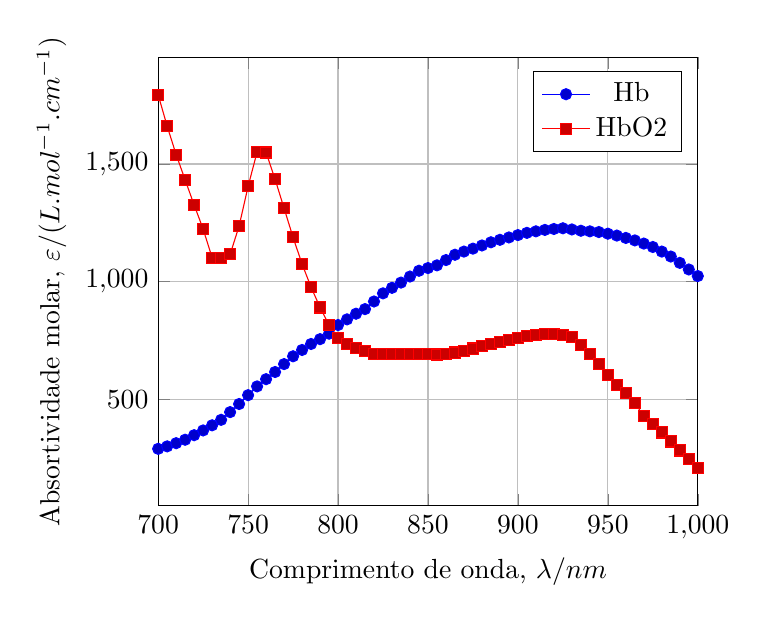
\begin{tikzpicture}
    \begin{axis}
        [
            grid = major,
            legend pos = north east,
            xlabel = {Comprimento de onda, $\lambda/\unit{nm}$},
            ylabel = {Absortividade molar, $\varepsilon/(\unit{L.mol^{-1}.cm^{-1}})$},
            xmin=700, xmax=1000,
            % ymax=7, ymax=1.1,
        ]
    \addplot coordinates
        {
            (650.0, 368.0)
            (655.0, 340.3)
            (660.0, 319.6)
            (665.0, 305.6)
            (670.0, 294.0)
            (675.0, 283.8)
            (680.0, 277.6)
            (685.0, 273.6)
            (690.0, 276.0)
            (695.0, 280.6)
            (700.0, 290.0)
            (705.0, 300.4)
            (710.0, 314.0)
            (715.0, 328.6)
            (720.0, 348.0)
            (725.0, 368.2)
            (730.0, 390.0)
            (735.0, 413.2)
            (740.0, 446.0)
            (745.0, 480.4)
            (750.0, 518.0)
            (755.0, 555.2)
            (760.0, 586.0)
            (765.0, 616.4)
            (770.0, 650.0)
            (775.0, 683.2)
            (780.0, 710.0)
            (785.0, 735.4)
            (790.0, 756.0)
            (795.0, 779.2)
            (800.0, 816.0)
            (805.0, 840.0)
            (810.0, 864.0)
            (815.0, 883.6)
            (820.0, 916.0)
            (825.0, 950.6)
            (830.0, 974.0)
            (835.0, 996.3)
            (840.0, 1022.0)
            (845.0, 1046.5)
            (850.0, 1058.0)
            (855.0, 1069.5)
            (860.0, 1092.0)
            (865.0, 1114.5)
            (870.0, 1128.0)
            (875.0, 1140.5)
            (880.0, 1154.0)
            (885.0, 1167.5)
            (890.0, 1178.0)
            (895.0, 1188.0)
            (900.0, 1198.0)
            (905.0, 1207.5)
            (910.0, 1214.0)
            (915.0, 1220.0)
            (920.0, 1224.0)
            (925.0, 1227.0)
            (930.0, 1222.0)
            (935.0, 1216.5)
            (940.0, 1214.0)
            (945.0, 1211.0)
            (950.0, 1204.0)
            (955.0, 1196.0)
            (960.0, 1186.0)
            (965.0, 1175.5)
            (970.0, 1162.0)
            (975.0, 1147.5)
            (980.0, 1128.0)
            (985.0, 1107.0)
            (990.0, 1080.0)
            (995.0, 1052.0)
            (1000.0, 1024.0)
        };
    \addplot coordinates
        {
            (650.0, 3750.0)
            (655.0, 3481.5)
            (660.0, 3227.0)
            (665.0, 3011.0)
            (670.0, 2795.0)
            (675.0, 2591.0)
            (680.0, 2408.0)
            (685.0, 2224.5)
            (690.0, 2052.0)
            (695.0, 1923.5)
            (700.0, 1794.0)
            (705.0, 1661.0)
            (710.0, 1540.0)
            (715.0, 1432.5)
            (720.0, 1326.0)
            (725.0, 1224.0)
            (730.0, 1102.0)
            (735.0, 1102.0)
            (740.0, 1116.0)
            (745.0, 1236.5)
            (750.0, 1405.0)
            (755.0, 1551.0)
            (760.0, 1549.0)
            (765.0, 1435.5)
            (770.0, 1312.0)
            (775.0, 1188.5)
            (780.0, 1075.0)
            (785.0, 977.04)
            (790.0, 890.79)
            (795.0, 815.89)
            (800.0, 761.70)
            (805.0, 733.70)
            (810.0, 717.10)
            (815.0, 703.95)
            (820.0, 693.79)
            (825.0, 693.39)
            (830.0, 693.00)
            (835.0, 692.70)
            (840.0, 692.39)
            (845.0, 691.89)
            (850.0, 691.29)
            (855.0, 690.75)
            (860.0, 694.29)
            (865.0, 698.95)
            (870.0, 705.79)
            (875.0, 716.15)
            (880.0, 726.39)
            (885.0, 734.90)
            (890.0, 743.60)
            (895.0, 752.70)
            (900.0, 761.79)
            (905.0, 768.59)
            (910.0, 774.60)
            (915.0, 778.20)
            (920.0, 777.39)
            (925.0, 774.50)
            (930.0, 763.79)
            (935.0, 730.25)
            (940.0, 693.39)
            (945.0, 650.79)
            (950.0, 602.20)
            (955.0, 561.70)
            (960.0, 525.60)
            (965.0, 484.35)
            (970.0, 429.30)
            (975.0, 395.80)
            (980.0, 359.69)
            (985.0, 321.45)
            (990.0, 283.19)
            (995.0, 245.05)
            (1000.0, 206.8)
        };
    \legend{\ce{Hb},\ce{HbO2}}
\end{axis}
\end{tikzpicture}